\documentclass[11pt]{article}\usepackage{geometry} \geometry{letterpaper, margin=25.4mm}
\usepackage{mathptmx}
\usepackage{layout}
\usepackage[blocks]{authblk}
\usepackage{titlesec}
\usepackage[english]{babel}
\usepackage{fancyhdr}
\usepackage{indentfirst}
\usepackage{hyperref}
\usepackage{array}
\usepackage{graphicx}
\usepackage{mathptmx} 
\usepackage[mathscr]{euscript}

\usepackage{slashbox}
\usepackage{pdfpages}

\usepackage{amsmath}
\usepackage{caption,subcaption,color}
\usepackage{makeidx}
\usepackage{multirow}
\usepackage{xspace}
\usepackage{tabularx}
\usepackage{rotating}
\usepackage{float}
\usepackage{amsmath,amssymb,pifont,bbold}
\usepackage{tikz}
\usetikzlibrary{trees}
\usetikzlibrary{decorations.pathmorphing}
\usetikzlibrary{decorations.markings}
\usetikzlibrary{arrows,shapes,patterns}
\usepackage{glossaries}
\usepackage{etoolbox}
\usepackage{bibunits}
\usepackage{sidenotes}
\usepackage{animate}
\usepackage{theorem}
\usepackage{enumitem}
\usepackage{booktabs}
\usepackage{mhchem}
\usepackage{lastpage}

\pagenumbering{arabic}
\pagestyle{fancy}
\fancyhead{}
\fancyfoot{}
\fancyhead[LO,LE]{\fontsize{8}{10}\selectfont \bf The 9TH European Review Meeting on Severe Accident Research (ERMSAR2019) \\ Clarion Congress Hotel, Prague, Czech Republic, March 18-20, 2019}
\fancyhead[RE,RO]{\fontsize{8}{10}\selectfont \bf Log Number: xxx \\~}
\renewcommand{\headrulewidth}{0pt}
\fancyfoot[RO,RE]{\fontsize{8}{10}\selectfont \bf \thepage/\pageref{LastPage}}

%\setlength{\parskip}{1em}

% \renewenvironment{abstract}{\global\setbox\absbox=\vbox\bgroup
%   \hsize=\textwidth\def\baselinestretch{1}%
%   \noindent\unskip\begin{center}\textbf{Abstract}\end{center}
%  \par\medskip\noindent\unskip\ignorespaces}
%  {\egroup}
 
\bibliographystyle{abbrv}

\newenvironment{legend}
{\tabular{r>{\small} p{0.9\textwidth}}}
{\endtabular}

\newcommand{\n}{\tabularnewline}
\newcolumntype{C}{>{\centering}X}
\newcolumntype{L}{>{\raggedright}X}
\newcolumntype{R}{>{\raggedleft}X}
\newcolumntype{M}[1]{>{\centering}m{#1}}

\newenvironment{remark}[1][\rule{1ex}{1ex} \textit{Nota Bene}]{\begin{trivlist}
\item[\hskip \labelsep {\bfseries #1}]}{\rule{1ex}{1ex} \end{trivlist}}


% notations
\newcommand{\T}{\texttt}
\newcommand{\M}[1]{{\mathbb #1}}
\newcommand{\Mb}[1]{{\mathbf #1}}
\newcommand{\Mc}[1]{{\mathcal #1}}
\newcommand{\Ms}[1]{{\mathcal{} #1}}
\newcommand{\Hi}[1]{\underline{#1}}

\newcommand{\Eq}[1]{Eq.~\ref{eq:#1}}
\newcommand{\Eqs}[2]{Eqs.~\ref{eq:#1} and~\ref{eq:#2}}
\newcommand{\Eqss}[3]{Eqs.~\ref{eq:#1},~\ref{eq:#2} and~\ref{eq:#3}}
\newcommand{\Eqsss}[4]{Eqs.~\ref{eq:#1},~\ref{eq:#2},~\ref{eq:#3} and~\ref{eq:#4}}
\newcommand{\Fig}[1]{Figure~\ref{fig:#1}}
\newcommand{\Figs}[2]{Figures~\ref{fig:#1} and~\ref{fig:#2}}
\newcommand{\Figss}[3]{Figures~\ref{fig:#1},~\ref{fig:#2} and~\ref{fig:#3}}
\newcommand{\Tab}[1]{Table~\ref{tab:#1}}
\newcommand{\Tabs}[2]{Tables~\ref{tab:#1} and~\ref{tab:#2}}
\newcommand{\Tabss}[3]{Tables~\ref{tab:#1},~\ref{tab:#2} and~\ref{tab:#3}}
\newcommand{\Sect}[1]{Section~\ref{sect:#1}}
\newcommand{\Sects}[2]{Sections~\ref{sect:#1}~and~\ref{sect:#2}}
\newcommand{\Sec}[1]{\Sect{#1}}
\newcommand{\App}[1]{Appendix~\ref{app:#1}}

\makeatletter
\patchcmd{\@maketitle}{\LARGE}{\fontsize{14}{17}\selectfont}{}{}
\makeatother

% notations
\newcommand{\functional}[2][\cdot]{\Mc{#2}\left[#1\right]}
\newcommand{\function}[2][\cdot]{#2\left(#1\right)}
\newcommand{\grad}[1]{\vec{\nabla} #1}
\newcommand{\dX}[1]{\frac{\partial #1}{\partial x}}
\renewcommand{\div}[1]{\vec{\nabla} \cdot #1}
\newcommand{\Lapl}[1]{\Delta #1}
\newcommand{\LaplX}[1]{\frac{\partial^2 #1}{\partial x^2}}
\newcommand{\domain}[1]{\Omega_{#1}}
\newcommand{\boundary}[1]{\partial \domain{#1}}
\newcommand{\interface}[1]{\Gamma_{#1}}

% notations
\newcommand{\formulaWithUnits}[2]{\begin{disarray}{lcr} #1 & ~~~ & \left[#2\right] \end{disarray}}
\newcommand{\formulaWithoutUnits}[2]{\begin{disarray}{lcr} #1 & ~~~ &  \end{disarray}}
\newcommand{\formula}[2]{\formulaWithUnits{#1}{#2}}
% phase change enthalpy / enthalphie de changement de phase ou chaleur latente
% J.kg^{-1}
\newcommand{\dEnthalpy}[2][\null]{\Delta h_{#2}^{\textrm{#1}}}
\newcommand{\dEnthalpyUnits}{\text{J.kg$^{-1}$}}
% specific heat capacity / capacité thermique massique
% J.kg^{-1}.K^{-1}
\newcommand{\heatCp}[2][\null]{Cp_{#2}^{\textrm{#1}}}
\newcommand{\heatCpUnits}{\text{J.kg$^{-1}$.K$^{-1}$}}
% mass flow rate / débit massique
% kg.s ^-1
\newcommand{\mFlowRate}[2][\null]{\dot{m}_{#2}^{\textrm{#1}}}
\newcommand{\mFlowRateUnits}{\text{kg.s$ ^{-1}$}}
% volumetric flow rate / débit massique
% m^3.s ^-1
\newcommand{\vFlowRate}[2][\null]{\dot{V}_{#2}^{\textrm{#1}}}
\newcommand{\vFlowRateUnits}{\text{m$^3$.s$ ^{-1}$}}
% power / puissance
% W
\newcommand{\power}[2][\null]{\dot{Q}_{#2}^{\textrm{#1}}}
\newcommand{\powerUnits}{\text{W}}
% mass power / puissance massique
% W.kg^-1
\newcommand{\massPower}[1]{\dot{q}_{#1}^{\textrm{mass}}}
\newcommand{\massPowerUnits}{\text{W.kg$^{-1}$}}
% volume power / puissance volumique
% W.kg^-1
\newcommand{\volPower}[1]{\dot{q}_{#1}^{\textrm{vol}}}
\newcommand{\volPowerUnits}{\text{W.m$^{-3}$}}
% heat flux / flux de chaleur
% W.m^-2
\newcommand{\heatFlux}[2][\null]{\phi_{#2}^{\textrm{#1}}}
\newcommand{\avHeatFlux}[2][\null]{\bar{\phi}_{#2}^{\textrm{#1}}}
\newcommand{\heatFluxUnits}{\text{W.m$^{-2}$}}
% surface
% m^{2}
\newcommand{\area}[2][\null]{S_{#2}^{\textrm{#1}}}
\newcommand{\areaUnits}{\text{m$^2$}}
% mass / mass
% kg
\newcommand{\mass}[2][\null]{m_{#2}^{\textrm{#1}}}
\newcommand{\massUnits}{\text{kg}}
% mass fraction / fraction massique
% 
\newcommand{\massFraction}[2][\null]{w_{#2}^{#1}}
\newcommand{\massFractionUnits}{}
% mass enthalpy / enthalpie massique
% 
\newcommand{\massEnthalpy}[2][\null]{h_{#2}^\textrm{#1}}
\newcommand{\massEnthalpyUnits}{\text{J.kg$^{-2}$}}
% pressure
% Pa
\newcommand{\pressure}[2][\null]{p_{#2}^{\textrm{#1}}}
\newcommand{\pressureUnits}{\text{Pa}}
% temperature
% K
\newcommand{\temperature}[2][\null]{T_{#2}^{\textrm{#1}}}
\newcommand{\temperatureUnits}{\text{K}}
% porosity / porosité
% none
\newcommand{\porosity}[2][\null]{\varepsilon_{#2}^{\textrm{#1}}}
% mass density / densité massique
% kg.m^{-3}
\newcommand{\massDensity}[2][\null]{\rho_{#2}^{\textrm{#1}}}
\newcommand{\massDensityUnits}{\text{kg.m$^{-3}$}}
% thermal conductivity / conductivité thermique
% W.m^{-1}.K^{-1}
\newcommand{\thermalCond}[2][\null]{\lambda_{#2}^{\textrm{#1}}}
\newcommand{\thermalCondUnits}{\text{W.m$^{-1}$.K$^{-1}$}}
% dynamic viscosity / viscosité dynamique
% Pa.s
\newcommand{\dynamicVisc}[2][\null]{\mu_{#2}^{\textrm{#1}}}
\newcommand{\dynamicViscUnits}{\text{Pa.s}}
% thermal expansion coefficient / coefficient de dilatation isobare
% K^{-1}
\newcommand{\thermalExp}[2][\null]{\beta_{#2}^{\textrm{#1}}}
\newcommand{\thermalExpUnits}{\text{K$^{-1}$}}
% convective heat transfer coeffcient / coefficient de transfert de chaleur convectif
% W.m^{-2}.K^{-1}
\newcommand{\thermalConv}[2][\null]{h_{#2}^{\textrm{#1}}}
\newcommand{\avThermalConv}[2][\null]{\bar{h}_{#2}^{\textrm{#1}}}
\newcommand{\thermalConvUnits}{\text{W.m$^{-2}$.K$^{-1}$}}
% Nusselt number / nombre de Nusselt
\newcommand{\Nu}[2][\null]{Nu_{#2}^{\textrm{#1}}}
% thermal conductivity / conductivité thermique
% W.m^{-1}.K^{-1}
\newcommand{\thermalDiff}[2][\null]{\alpha_{#2}^{\textrm{#1}}}
\newcommand{\thermalDiffUnits}{\text{W.m$^{-1}$.K$^{-1}$}}
% dynamic viscosity / viscosité dynamique
% Pa.s
\newcommand{\cinematicVisc}[2][\null]{\nu_{#2}^{\textrm{#1}}}
\newcommand{\cinematicViscUnits}{\text{Pa.s}}
% emissivity
%
\newcommand{\emissivity}[2][\null]{\epsilon_{#2}^{\textrm{#1}}}
\newcommand{\emissivityUnits}{\text{-}}

\newcommand{\property}[2][\null]{p^{#1}_{#2}}
\newcommand{\avProperty}[2][\null]{\bar{p}^{#1}_{#2}}

\newcommand{\flux}[2][\null]{\vec{\varphi}^{#1}_{#2}}
\newcommand{\avFlux}[2][\null]{\bar{\varphi}^{#1}_{#2}}
\newcommand{\massSource}[2][\null]{\dot{s}^{#1}_{#2}}
\newcommand{\avMassSource}[2][\null]{\bar{\dot{S}}^{#1}_{#2}}

\newcommand{\avMassFraction}[2][\null]{\bar{w}_{#2}^{#1}}
\newcommand{\massFlux}[2][\null]{\vec{J}^{#1}_{#2}}
\newcommand{\avMassFlux}[2][\null]{\bar{J}^{#1}_{#2}}
\newcommand{\elementMassFraction}[2][\null]{\bar{f}_{#2}^{#1}}

\renewcommand{\massEnthalpy}[2][\null]{h^{#1}_{#2}}
\newcommand{\avMassEnthalpy}[2][\null]{\bar{h}^{#1}_{#2}}
\renewcommand{\heatFlux}[2][\null]{\phi^{#1}_{#2}}
\renewcommand{\avHeatFlux}[2][\null]{\bar{\phi}^{#1}_{#2}}
\newcommand{\avMassPower}[1]{\dot{q}_{#1}^{\textrm{mass}}}
\newcommand{\avTemperature}[2][\null]{\bar{\temperature{}}_{#2}^{\textrm{#1}}}

\newcommand{\speciesSet}[1][\null]{\Mc{S}_{#1}}
\newcommand{\elementSet}[1][\null]{\Mc{E}_{#1}}
\newcommand{\phaseSet}[1][\null]{\Mc{P}_{#1}}

\newcommand{\OPSet}[1][\null]{\underline{\phi}_{#1}}


\renewcommand\Authfont{\bfseries}
\setlength{\affilsep}{0pt}
\titleformat{\section}{\bfseries}{\thetitle.}{1em}{\MakeUppercase}
\titleformat{\subsection}{\normalfont\bfseries}{\thetitle.}{1em}{}
\titleformat{\subsubsection}{\normalfont\bfseries}{\thetitle.}{1em}{}

\begin{document}

\title{\vspace{-1em}\bf \MakeUppercase{Consistent use of CALPHAD data for in-vessel corium pool modeling:} \\ \MakeUppercase{some analytical and practical considerations}}
\date{}

\author{R. Le Tellier}
\author{B. Habert}  
\author{V. Tiwari}  
\affil{CEA, DEN, DTN/SMTA/LMAG, Cadarache \\
  F-13108 Saint Paul-lez-Durance, France \\
  \underline{romain.le-tellier@cea.fr}, benoit.habert@cea.fr, vaishnvi.tiwari@cea.fr}
\author{N. Bakouta}
\affil{EDF Lab Paris-Saclay \\
  7, boulevard Gaspard Monge \\
  F-91120, Palaiseau, France \\
  nikolai.bakouta@edf.fr}

\maketitle

\thispagestyle{fancy}

\section*{Abstract} 

\section*{\hfill Keywords}
\hfill \texttt{in-vessel corium, CALPHAD, thermodynamic properties, tabulation, interpolation}

%%%%%%%%%%%%%%%%%%%%%%%%%%%%%%%%%%%%%%%%%%%%%%%%%%%%%%%%%%%%%%%%%%%%%%%%%%%%%
\section{Introduction}
%%%%%%%%%%%%%%%%%%%%%%%%%%%%%%%%%%%%%%%%%%%%%%%%%%%%%%%%%%%%%%%%%%%%%%%%%%%%%

This work pertains to the modeling of in-vessel corium pool within the framework of Severe Accident studies for Light Water Reactors (LWRs). Considering in particular ``In-Vessel Retention'' (IVR) safety strategies, a key element is the phenomenology associated with a corium pool that can be formed after the loss of the primary coolant and the induced core degradation. Indeed, the heat flux from the corium pool to the vessel wall determines the chances of success of a reactor pit reflooding strategy (``External Reactor Vessel Cooling'' ERVC). The behavior of a corium pool results from the combination of two main types of phenomena. While, the associated thermochemistry defines the segregation of the pool in different phases (both liquid and solid), thermohydraulics finally determines through natural convection (that may be laminar or turbulent depending on the size) the heat flux at the pool interface.

In this context, code cross-comparisons \cite{Bakouta2015} performed by CEA and EDF on the stratified in-vessel corium pool models of PROCOR (CEA, see \cite{LeTellier2015}) and EDF proprietary versions of MAAP4 \cite{maap4} and MAAP5 \cite{maap5} (indistinctly referred to as MAAP-EDF in the remainder) have shown that an important source of discrepancy is related to the associated thermodynamic representation of the sub-oxidized corium-steel system. The PIRT (Phenomena Identification Ranking Table) developed in the frame of the H2020 European project IVMR (In-Vessel Melt Retention) has also pointed out the prime importance of gaining knowledge for a more detailed modeling of the thermochemical peculiarities (e.g. liquid miscibility gap) of the corium-steel system. Indeed, the modeling of corium-steel thermochemical interactions in codes treating of in-vessel corium behavior is rather recent\footnote{For instance, first efforts for constructing transient stratification models can be traced back to the OECD MASCA program in the early 2000's \cite{Tsurikov2007}.} and is still very incomplete \cite{Carenini2018}. In particular, the recent results of the CORDEB experimental program \cite{Almjashev2018} have clearly shown the requirement for further studies regarding the thermochemical interactions between molten steel and suboxidized corium crust. 

In addition to thermochemical modeling aspects related to phase-component partitioning (e.g. for the liquid phases and the related phase stratification), such thermodynamic information is needed for the closures of thermal models, in particular in terms of enthalpy-temperature relations as a function of the composition for energy conservation equations.

As thermochemical models are introduced in codes that historically dealt only with corium thermalhydraulics, an issue is raised pertaining to the consistency of the corium-steel system thermodynamic representation underlying the different models or closures. In the case of the MAAP-EDF code, it was shown in \cite{Bakouta2015} that the native MAAP ``Equation-Of-State'' (EOS) that provides the closures (the specific enthalpy, the liquidus temperature and so on for a given material composition) to energy balance equations written in enthalpy is inconsistent with the findings of the MASCA project regarding corium-steel thermochemical interactions and, consequently, with the liquid phases stratification model proposed in \cite{LeTellier2014} and introduced in MAAP-EDF. It leads to erroneous temperatures at the interface between the liquid corium pool layers and the surrounding oxidic crust. 

In order to solve this consistency issue, a single, as exhaustive as possible, thermodynamic representation of the system should be used throughout all the different models and closures. Severe accident dedicated thermodynamic databases constructed by the CALPHAD method \cite{Lukas2007} offer such a representation. Actually, various thermochemical models that are used for in-vessel corium behavior are based in one way or the other on thermodynamical description of the corium system through databases obtained with the CALPHAD approach \cite{Lukas2007}. Such databases are constructed in terms of mathematical models (with adjustable parameters fitted on experimental data \cite{Barrachin2004, Gueneau2015}) that represent the Gibbs energy of the different phases for low-order systems (in practice, binary and ternary systems). This information, through extrapolation, is used to calculate the Gibbs energy of higher-order systems in such a way that these databases, combined with a Gibbs energy minimizer code, can be used to calculate the thermodynamical properties of a system at isothermal equilibrium. Gibbs energy phase models in such databases also offer the possibility of extrapolating outside the thermodynamic stability range and consequently can be used in kinetic modeling of phase transformations.

In \cite{Tiwari2018}, as a first step towards a CALPHAD-based EOS for in-vessel corium, a preliminary study was carried out on a simple plane front solidification model for the ternary U-O-Zr system and the results have confirmed the feasibility of using the CALPHAD database to obtain thermodynamically consistent for the conservation equations. 

In this preliminary work, two major ``simplifications'' were made and require further analysis. On the one hand, under the hypotheses of this solidification model, both liquid and solid regions are monophasic in such a way that they can be directly related to the phases described in the CALPHAD database. In the general case, CALPHAD data should be supplemented by phase segregation hypotheses and models for the construction of the desired EOS. %It should be emphasized that these hypotheses should be made, as far as possible, consistent with in-vessel corium associated thermochemical models to which the thermal balance is coupled with. 
On the other hand, this solidification model, from the point of view of CALPHAD-derived quantities (including thermodynamic equilibria), makes direct use of a Gibbs energy minimizing code (the Open-Calphad code as interfaced in PROCOR, see \cite{Sundman2016}). Considering the complete modeling of in-vessel corium, for the sake of robustness and performances, this direct approach appears impractical. As a consequence, tabulation and interpolation strategies regarding the CALPHAD-based thermodynamic properties (e.g. \cite{Saad2015}) have to be envisaged.

This paper is focused on these two differents aspects associated with the consistent and practical use of CALPHAD data for in-vessel corium pool modeling.
First, different segregation hypotheses that can be made when constructing such an EOS are discussed and analyzed in \Sect{analytical} for the steel-corium system on a simple test case. Then, \Sect{practical} reports ongoing developments regarding the sampling, storage and interpolation of CALPHAD-based thermodynamic properties for the EOS construction. Conclusions and perspectives are proposed in \Sect{concl}.

%%%%%%%%%%%%%%%%%%%%%%%%%%%%%%%%%%%%%%%%%%%%%%%%%%%%%%%%%%%%%%%%%%%%%%%%%%%%%
\section{Comparing different segregation hypotheses for constructing an in-vessel corium EOS} \label{sect:analytical}
%%%%%%%%%%%%%%%%%%%%%%%%%%%%%%%%%%%%%%%%%%%%%%%%%%%%%%%%%%%%%%%%%%%%%%%%%%%%%


\subsection{Energy conservation equations formulation} \label{sect:cons_eq}

For the sake of clarity, let us first recall from the general formulation of mass, species mass fractions and energy conservation equations that is relevant for in-vessel corium related integral models. The reader is referred to classical textbooks for more details (e.g. Appendices A\&B of \cite{Kaviany2011}).

The spatial domain is decomposed in different spatial zones $\domain{n}$ and the boundary of $\domain{n}$, denoted $\boundary{n}$ is split according to $\boundary{n} = \bigcup_{m \in \Mc{N}(n)} \interface{n,m} + \interface{n,\textrm{ext}}$ where $\interface{n,m}=\interface{m,n}$ represents the interface of area $\area{\interface{n,m}}$ between domains $n$ and $m$ while $\interface{n,\textrm{ext}}$ is the part of $\boundary{n}$ of area $\area{\interface{n,\textrm{ext}}}$ that lies on the system boundary. $\Mc{N}(n)$ denotes the set indices corresponding to regions that are neighbor of $\domain{n}$.

Considering the notations given in \Tab{notations_eq}, the mass conservation equation for $\domain{n}$  is simply: 
\begin{equation} 
 \frac{d\mass{n}}{dt}  + \sum_{m \in  \Mc{N}(n)} \dot{m}_{\interface{n,m},n} + \dot{m}_{n, \textrm{ext}} = 0 \label{eq:mce_m}
\end{equation}
The associated interface conditions on $\interface{n,m}$ are given by:
\begin{equation}
 \dot{m}_{\interface{n,m},n}+\dot{m}_{\interface{n,m},m} = 0 \label{eq:ie_m}
\end{equation}

Then, for any intensive property $p$ (units [p].kg$^{-1}$), conservation over $\domain{n}$ can be written as:
 \begin{equation}
  \frac{d}{dt} \left( \avProperty{n} \mass{n} \right) + \sum_{m \in  \Mc{N}(n)} \left(\avFlux[p]{\interface{n,m},n} \area{\interface{n,m}} + \avProperty{\interface{n,m},n} \dot{m}_{\interface{n,m},n}\right) + \avFlux[p]{n, \textrm{ext}} \area{\interface{n,\textrm{ext}}} + \avProperty{n, \textrm{ext}} \dot{m}_{n, \textrm{ext}} = \avMassSource[p]{n} \mass{n} \label{eq:mce3}
\end{equation}
while the associated interface conditions can be formulated as:
\begin{equation}
 \avProperty{\interface{n,m},n} \dot{m}_{\interface{n,m},n} + \avProperty{\interface{n,m},m} \dot{m}_{\interface{n,m},m} + \left(\avFlux[p]{\interface{n,m},n} +\avFlux[p]{\interface{n,m},m}\right) \area{\interface{n,m}} = 0 \label{eq:ie2}
\end{equation}
\Eq{ie2} is sometimes referred to as Kotchine's theorem, written here, for the sake of simplicity without any singular term (\textit{i.e.} no accumulation, generation or transport of property $p$ on the interface).

In particular, when considering in-vessel corium model, such equations are written for $p=\massEnthalpy{}$, the mass enthalpy, in such a way that \Eq{mce3} is the energy conservation equation for $\domain{n}$ (neglecting viscous dissipation and the effect of the pressure material derivative)\footnote{These assumptions are compatible with the Boussinesq approximation of fluid dynamics often used for treating corium natural convection.}. Along with mass and energy conservation, as discussed in the introduction, corium complex thermodynamics requires to keep track of the composition of $\domain{n}$. Here, we will consider that this is achieved by writing conservation equation with $p=\massFraction[j]{}$, the mass fraction of stoichiometric species $j$ ($j\in \speciesSet$). The associated element set is denoted $\elementSet$.

\begin{table}[H]
\caption{notations associated with integral conservation equations} \label{tab:notations_eq}
\vskip -\baselineskip
\begin{small}
\begin{tabularx}{1.0\textwidth}{LLl} \n \hline
notation & units & \multicolumn{1}{c}{description} \n \hline \hline
$\mass{n}$ & kg & mass of $\domain{n}$ \n
$\dot{m}_{\interface{n,m},n}$  & kg.s$^{-1}$ & total mass flow rate through $\interface{n,m}$ (counted positive from $\domain{n}$ to $\domain{m}$) \n
$\dot{m}_{n, \textrm{ext}}$  & kg.s$^{-1}$ & total mass flow rate through $\interface{n,\textrm{ext}}$ (counted positive from $\domain{n}$ to the outside) \n
$\avProperty{n} \mass{n}$ & [p].kg$^{-1}$ & mass averaged property $p$ over $\domain{n}$ \n
$\avMassSource[p]{n}$ & [p].kg$^{-1}$.s$^{-1}$ & mass averaged source of property p in $\domain{n}$ \n
$\avProperty{\interface{n,m},n}\dot{m}_{\interface{n,m},n}$ & [p].s$^{-1}$ & transfer rate of property p from $\domain{n}$ to $\domain{m}$ associated with mass transfer through $\interface{n,m}$ \n
$\avProperty{n, \textrm{ext}} \dot{m}_{n, \textrm{ext}}$ & [p].s$^{-1}$ & transfer rate of property p out of $\domain{n}$ associated with mass transfer through $\interface{n,\textrm{ext}}$ \n
$\avFlux[p]{\interface{n,m},n}$ & [p].m$^{-2}$.s$^{-1}$ & average flux of property p through $\interface{n,m}$ (counted positive from $\domain{n}$ to $\domain{m}$) \n 
$\avFlux[p]{n, \textrm{ext}}$ & [p].m$^{-2}$.s$^{-1}$ & average flux of property p through $\interface{n,\textrm{ext}}$ (counted positive from $\domain{n}$ to the outside) \n \hline
\end{tabularx}
\end{small}
\end{table}


\subsection{Closure requirements} \label{sect:req}

For any spatial zone spatial $\domain{}$, the closure of energy conservation equations requires enthalpy-temperature relations and, in the framework of multicomponent systems, the dependence of such relations to chemical composition is of importance (see \cite{Schneider1991}) and should be treated adequately. 

\begin{remark}
In the remainder, the pressure possible dependence of thess functions will be neglected and we will consider that the corium materials density is not affected by pressure. This is a reasonable assumption for corium liquid phases compatible with the Boussinesq approximation of fluid dynamics (see \cite{Hills1991}) often used for modeling natural convection in this context.
\end{remark}

In this framework, for a given thermodynamic system, the enthalpy-temperature relations may be described in a general way by a function referred to as an ``Equation-Of-State'' (EOS) and described by:
\begin{equation}
 \Mc{H}: \avTemperature{}, \left(\avMassFraction[j]{}\right)_{j\in \speciesSet} \rightarrow  \left(\omega_\gamma, \avMassEnthalpy{\gamma}, \left(\massFraction[j]{\gamma}\right)_{j\in \speciesSet}\right)_{\gamma \in \phaseSet} \label{eq:eos}
\end{equation}
where $\phaseSet$ is the set of phases in zone $\domain{}$ and, for each phase $\gamma \in \phaseSet$, $\omega_\gamma$ is the mass fraction, $\avMassEnthalpy{\gamma}$ the corresponding specific enthalpy (J/kg) while $\left(\massFraction[j]{\gamma}\right)_{j\in \speciesSet}$ gives the composition of $\domain{}$ in terms of the different phases ($\omega_\gamma$ is the mass fraction of phase $\gamma$ while $\left(\massFraction[j]{\gamma}\right)_{j\in \speciesSet}$ gives its composition). The average specific enthalpy is then given by $\avMassEnthalpy{} = \displaystyle \sum_{\gamma \in \phaseSet} \omega_\gamma \avMassEnthalpy{\gamma}$.

From $\Mc{H}$, a reciprocal temperature-enthalpy relation can be obtained and is denoted:
\begin{equation}
\Mc{T}: \avMassEnthalpy{}, \left(\avMassFraction[j]{}\right)_{j\in \speciesSet} \rightarrow \avTemperature{}, \left(\omega_\gamma, \left(\avMassFraction[j]{\gamma}\right)_{j\in \speciesSet}\right)_{\gamma \in \phaseSet}
\end{equation}
In the general case, for given $\avMassEnthalpy{}$ and $\left(\avMassFraction[j]{}\right)_{j\in \speciesSet}$, $\avTemperature{}$ is obtained by solving the following non-linear root-finding problem: 
\begin{equation}
 \text{find } \avTemperature{} \text{ such that }\Mc{H}\left[\avTemperature{}, \left(\avMassFraction[j]{}\right)_{j\in \speciesSet}\right] = \avMassEnthalpy{} \label{eq:t(h)}
\end{equation}

\subsection{Relations provided by CALPHAD data}

In CALPHAD-type thermodynamic databases, the Gibbs energy of each phase is described by a model depending on the state variables \cite{Lukas2007}. The Compound Energy Formalism (CEF) (see \cite{Hillert2001}), as used for instance in the Open-Calphad code \cite{Sundman2015}, encompasses many different kinds of models. In this formalism, the different constituents of a phase (neutral atoms, ions, vacancies, etc.) are distributed in one or more thermodynamic sublattices where they mix according to the classical solution theory (ideal or non-ideal model) with different interaction parameters in different sublattices. Each sublattice $s$ is defined by its number of sites $a^{(s)}$ and the set of constituents that occupy these sites. This general formalism describes the Gibbs energy per formula unit, $G_M$, of a phase $\gamma$ as:
\begin{equation}
 \Mc{G}_{M}^{\gamma}: \temperature{}, \pressure, \left(y_{k}^{(s)}\right)_{k,s} \rightarrow G
\end{equation}
where $T$ is the temperature (K), $p$ is the pressure (Pa) and $y_{k}^{(s)}$ is the molar fraction of constituent $k$ on sublattice $s$ with $\sum_k y_{k}^{(s)} = 1$. 

From there, the specific Gibbs energy (J/kg) can be obtained as:
\begin{equation}
 \Mc{G}^{\gamma}: \temperature{}, \pressure, \left(y_{k}^{(s)}\right)_{k,s} \rightarrow \Mc{G}_{M}^{\gamma}\left(\temperature{}, \pressure, \left(y_{k}^{(s)}\right)_{k,s}\right) / \sum_i \sum_s a^{(s)} \sum_k M_i S_i(k) y_{k}^{(s)} \label{eq:G1}
\end{equation}
where $S_i(k)$ is the stoichiometric coefficient of component $i$ in constituent $k$ and $M_i$ is the molar mass of component $i$. The denominator of \Eq{G1} represents the mass associated with one per formula unit.

The associated specific enthalpy function is then:
\begin{equation}
 \Mc{H}^{\gamma}: \temperature{}, \pressure, \left(y_{k}^{(s)}\right)_{k,s} \rightarrow H = \Mc{G}^{\gamma}\left(\temperature{}, \pressure, \left(y_{k}^{(s)}\right)_{k,s}\right) + T \Mc{S}^{\gamma}\left(\temperature{}, \pressure, \left(y_{k}^{(s)}\right)_{k,s}\right)  \label{eq:Hm1}
\end{equation}
where the specific entropy function is given by:
\begin{equation}
\Mc{S}^{\gamma}: \temperature{}, \pressure, \left(y_{k}^{(s)}\right)_{k,s} \rightarrow S = -\left.\frac{\partial \Mc{G}^{\gamma}}{\partial T}\right|_{\pressure, \left(y_{k}^{(s)}\right)_{k,s}} \left(\temperature{}, \pressure, \left(y_{k}^{(s)}\right)_{k,s}\right)
\end{equation}

As a consequence, for a given phase $\gamma$ described in a CALPHAD database, an enthalpy-temperature relation is directly given by the thermodynamic model for this phase in the database. In some thermodynamic softwares including Open-Calphad, it is possible to access such information.
It is very important to note that, in terms of composition variation, this function is defined in terms of the variables $\left(y_{k}^{(s)}\right)_{k,s}$ that depends on the phase model through its description in sublattice constituents.

In practice, for corium CALPHAD databases, only the gas phase is modeled as dependent on pressure; as a consequence, in the remainder where we focus on liquid and solid phases, the pressure variable will be omitted.

\subsection{Bridging the gap} \label{sect:gap}

As discussed in the introduction, the enthalpy-temperature relations (\Eq{Hm1}) as obtained from CALPHAD data are an interesting starting point in order to construct an EOS for energy conservation equations, see for instance \cite{Voller2006,Du2007}. In particular, in the framework of corium behavior modeling, such CALPHAD data are already in use in thermochemical models through equilibrium calculations and, in \cite{Tiwari2018}, a corium solidification model for the ternary U-O-Zr system making an extensive use of U-O-Zr CALPHAD data was successfully tested. It has confirmed the feasibility of using the CALPHAD database to obtain thermodynamically consistent closures for the conservation equations in terms of interface conditions associated with a local equilibrium hypothesis and enthalpy-temperature relations as a function of composition. Regarding the latter point, under the hypotheses of this model, the two spatial zones (liquid and solid) were known to be monophasic in such a way that the enthalpy-temperature relations were directly provided by two $\Mc{H}^{\gamma}$ functions without any complication.

However, in the general case, an EOS given by \Eq{eos} has to describe configurations where the spatial $\domain{}$ is multiphasic; in the context of integral corium models, such cases occur when:
\begin{itemize}
\item the temperature of a domain $\avTemperature{}$ falls below $\Mc{T}_{liq}\left(\avMassFraction[j]{}\right)_{j\in \speciesSet}$ (the liquidus temperature associated with the average composition) \textit{i.e.} a solid phase appears along with the liquid phase. In this case, solidification hypotheses are needed to bridge the gap between CALPHAD enthalpy-temperature relations for the different liquid and solid phases and the EOS that has to provide the species phase partitioning;
\item the average composition of the spatial domain $\left(\avMassFraction[j]{}\right)_{j\in \speciesSet}$ is in a miscibility gap region \textit{i.e.} from the point of view of the thermodynamic equilibrium, two immiscible phases (with the same description in terms of phase model in CALPHAD database but different compositions) are expected. In this case, additional hypotheses regarding this phase decomposition are needed for the construction of the EOS.
\end{itemize}
In a general way, CALPHAD data should be supplemented by phase segregation hypotheses and models for the construction of the desired EOS. It should be emphasized that these hypotheses should be made, as far as possible, consistent with thermochemical models to which the thermal model under consideration is coupled with. This is not a trivial matter and it is the main issue that was raised regarding MAAP-EDF in-vessel corium modeling because of the clear inconsistency between the ``native'' MAAP EOS and the hypotheses of the stratification kinetic model introduced in MAAP-EDF. 

\begin{remark}
From the conservation equations point of view, we have considered that the composition of a spatial zone is described in terms of species through $\left(\avMassFraction[j]{}\right)_{j\in \speciesSet}$. It is the case, for instance, in PROCOR and TOLBIAC-ICB \cite{Spindler2006} codes where physical properties such as density or conductivity are obtained from mixing laws applied to species density functions of temperature. 
As a consequence, in the general case, $\Mc{H}^{\gamma}$, function of $y_{k}^{(s)}$, cannot be used directly for the EOS construction and a ``conversion'' is needed. In the remainder, for the sake of simplicity, we will restrict ourselves to CALPHAD models with only one sublattice for which the constituents are stoichiometric species. In particular, this is the case for the non-ideal associate modeling used in the NUCLEA database \cite{Cheynet2002} for the phases of interest for in-vessel corium in the range of compositions and temperatures considered in \Sect{num}.
\end{remark}

\subsection{Numerical tests on possible segregation hypotheses} \label{sect:num}

We report here some tests that have been carried out in the framework of the PROCOR platform for testing different segregation hypotheses on a very simple case. The CALPHAD numerical tool that has been used is Open-Calphad through an interface in PROCOR (\cite{Sundman2016}). CALPHAD data that have been used are limited to $\elementSet = \left\{U,O,Zr,Fe\right\}$ elements and are taken from the NUCLEA'09 database. In this work, the temperature that is considered is between $[1800, 3100]$K and for the composition range of interest, only the liquid phase (denoted \T{LIQUID}) and the solid face-centered cubic (U,Zr)O$_{2-x}$ phase (denoted \T{C1\_FCC}) have been considered. Both phases are described by a non-ideal associate model based on the following stoichiometric species as constituents $\speciesSet = \left\{ U, UO_2, Zr, ZrO_2, Fe, Fe_2O_3, FeO, O \right\}$.

\begin{remark}{} 
Actually, below 2000K, solid phases other than \T{C1\_FCC} can be stable. In particular, when the temperature is lowered, the next solid phases to be formed are the tetragonal (Zr,U)O$_{2-x}$ phase (\T{TET(OXIDE)}) and the $\alpha$-Zr(O) phase (\T{HCP\_A3}) depending on the solidification path.
\end{remark}

\subsubsection{Test case description}

From the point of view of the conservation equations introduced in \Sect{cons_eq}, we consider here the situation of a single spatial domain with adiabatic boundary conditions and an external mass flow rate \textit{i.e} conservation equations reduce to:
\begin{eqnarray}
 \frac{d\mass{}}{dt} + \dot{m}_{\textrm{ext}} &=& 0 \label{eq:bulk_m1}\\
 \frac{d}{dt} \left( \avMassFraction[j]{} \mass{} \right) + \avMassFraction[j]{\textrm{ext}} \dot{m}_{\textrm{ext}} &=& 0 \label{eq:bulk_w1} \\
 \frac{d}{dt} \left( \avMassEnthalpy{} \mass{} \right) + \avMassEnthalpy{\textrm{ext}} \dot{m}_{\textrm{ext}} &=& 0  \label{eq:bulk_h1}
\end{eqnarray}

The domain is initially homogeneous and corresponds to a mass $\mass{ox}$ of suboxidized in-vessel corium material defined by its composition $\left(\massFraction[j]{ox}\right)_{j\in \speciesSet}$ in terms of its U/Zr molar ratio $R_{U/Zr}$ and Zr molar oxidation degree $C_{Zr}$ and its initial temperature $\temperature{ox} > \Mc{T}_{liq}\left(\massFraction[j]{ox}\right)_{j\in \speciesSet}$. The associated specific enthalpy is denoted $\massEnthalpy{ox}$.

The transient then consists in adding steel material in the domain: $- \dot{m}_{\textrm{ext}} = \dot{m}_{steel} >0$ at constant temperature $\temperature{steel}$. In these calculations, steel is considered as pure iron. The steel specific enthalpy is denoted $\massEnthalpy{steel}$.

Then, \Eqss{bulk_m1}{bulk_w1}{bulk_h1} are time-integrated and expressed in terms of $x_{steel}$ (defined by $\mass{steel} = \int \dot{m}_{steel} dt {\buildrel\rm def\over=} x_{steel}\mass{ox}$) as:
\begin{eqnarray}
 \mass{} &=& \mass{ox} \left(1 + x_{steel}\right) \\
 \mass{} \avMassFraction[j]{} &=& \mass{ox} \left(\massFraction[j]{ox} + \massFraction[j]{steel} x_{steel}\right) \\
 \mass{} \avMassEnthalpy{} &=& \mass{ox} \left(\massEnthalpy{ox} + \massEnthalpy{steel} x_{steel}\right)
\end{eqnarray}
This simple sequence is used to compare different EOS $\Mc{T}\left(\avMassEnthalpy{}, \left(\avMassFraction[j]{}\right)_{j\in \speciesSet}\right)$ in terms of $\avTemperature{}$, $\left(\omega_\gamma, \left(\avMassFraction[j]{\gamma}\right)_{j\in \speciesSet}\right)_{\gamma \in \phaseSet}$ as a function of $x_{steel}$. The liquidus temperature $\temperature{liq} = \Mc{T}_{liq}\left(\avMassFraction[j]{}\right)_{j\in \speciesSet}$ is also evaluated. In this sequence, the temperature is always above the steel liquidus temperature. 

%\begin{remark}{}
%In late 2016, CEA and EDF have used such a benchmark to compare different numerical tools. This joint work will be the subject of a technical report by EDF early 2017. In the present report, we only give and discuss results obtained by CEA and focus on the modeling aspects related to phase segregation in the EOS. In addition, in the EDF-CEA benchmark, three different cases where the oxidation degree of the corium and the steel temperature were varied have been treated while in the remainder, we will present and discuss only one case as the observations in terms of segregation hypotheses are similar.
%\end{remark}

\subsubsection{Segregation hypotheses for constructing the EOS} 

The following segregation modeling aspects that lead to different EOS are to be discussed:
\begin{enumerate}
 \item corium-steel chemical interaction: in addition to the case where corium-steel is treated thermodynamically as a multicomponent system (the U-O-Zr-Fe system in our simulations), the ``extreme'' case where suboxidized corium (U-O-Zr) and steel (Fe) are treated as two independent chemical systems without any interaction is considered. This latter assumption is the underlying one in codes that do not include models for the evaluation of the thermochemistry in the molten pool even for the equilibrium \cite{Carenini2019a}.
 
 \item solidification path: the two ``extreme'' cases of the lever-rule and Scheil\-/Gulliver model \cite{Scheil1942}, have been considered. In both closure relations, uniform solute distribution in the liquid is assumed while diffusion in the solid is considered as infinitely fast (resp. slow) for the lever-rule (resp. Scheil\-/Gulliver) method. Note that intermediate approaches where the diffusion in the solid is assumed either to be infinitely fast or slow depending on the component and the solid phase can be formulated (see, for instance, \cite{Chen2002,Schaffnit2015,Kozeschnik2007} for the solidification of steel modeling). In addition, when the initial system above the liquidus temperature is in the liquid miscibility gap, two ``extreme'' hypotheses can be made regarding the solidification path of the two liquids: either, the liquid phases are considered to be always in equilibrium (\textit{i.e.} inter-liquid mass transfer is fast in comparison with the solidification process) or, their solidification 
paths are considered as independent (if the cooling rate is sufficiently high, the inter-liquid mass transfer can be neglected).
 
 \item liquid-liquid separation: if corium-steel chemical interaction is considered, the liquid separation into two phases at thermodynamic equilibrium (due to the liquid miscibility gap in the U-O-Zr-Fe system) has to be dealt with. In the context of such an EOS, two extreme cases will be considered: either the liquid separation is infinitely fast in such a way that the liquid separation is given by the thermodynamic equilibrium or the liquid separation is infinitely slow.
\end{enumerate}
Note that we have only considered options regarding phase separation that provide direct closure relations for constructing the EOS without introducing additional variables subject to differential equations. When considering integral models (such an in PROCOR), this is a requirement. Even in the context of mesh-based models, so-called sub-cell models are often limited to such closures. For instance, in the context of an Eulerian macrosegregation modeling for alloy solidification, supplementary relationships based on the lever-rule or Scheil\-/Gulliver models are used in \cite{Du2007} to close the equation system.
 
For the numerical results presented hereafter, we have taken an initial suboxidized corium composition typical of French PWRs with $R_{U/Zr}=1.2$ with a low Zr molar oxidation degree $C_{Zr}=0.32$ (when varying the accident scenario, 0.3 is typically the lowest value of $C_{Zr}$ obtained from calculations of the core degradation and corium relocation in the lower head, see \cite{Seiler2014}). In addition, the temperatures are $\temperature{ox}=2900$K and $\temperature{steel}=1850$K while $x_{steel}$ discrete sequence is given by $x_{steel} = 0.05i$ with $0 \le i \le 20$. For the set of input parameters selected, one can expect three possible phases: one ``oxidic'' liquid phase (denoted \textit{``liquid,ox''}), one ``metallic'' liquid phase (denoted \textit{``liquid, met''}) and one ``oxidic'' solid phase (denoted \textit{``solid''}).

The different cases that are compared are summarized in \Tab{eos} in terms of segregation hypotheses. Not all possible option combinations have been tested; the different options have been tested in a one-at-a-time approach based on a reference case given by \T{equilibrium} computational case. Regarding these different options, one can note that:
\begin{itemize}
 \item while $x_{steel}$ is sufficiently low (in this case, $< 0.15$) in order to have $\bar{\temperature{}} \ge \temperature{liq}$, \T{equilibrium}, \T{Scheil\-/Gulliver} and \T{independent solidification} options are equivalent;
 \item when $x_{steel}$ is high enough (in this case, $\ge 0.45$) in such a way that the liquid oxidic phase has vanished, \T{equilibrium} and \T{single liquid equilibrium} are equivalent.
\end{itemize}

\begin{table}[H]
\renewcommand{\arraystretch}{1.3}
\caption{Computational cases description in terms of segregation hypotheses} \label{tab:eos}
\begin{scriptsize}
 \begin{tabularx}{\textwidth}{|l|l|C|C|C|C|} \cline{3-6}
 \multicolumn{1}{c}{} &  \multirow{3}{*}{} & \multicolumn{4}{c|}{segregation options} \n \cline{3-6}
 \multicolumn{1}{c}{} &                    & corium-steel & \multicolumn{2}{c|}{solidification hypotheses} & liquid \n \cline{4-5}
 \multicolumn{1}{c}{} &                    & interaction  & path & inter-liquid transfer$^\dagger$         & separation$^\ddagger$ \n \hline
  \multirow{10}{*}{\rotatebox{90}{computational case}}
  & \T{equilibrium} & \multirow{2}{*}{yes} & \multirow{2}{*}{lever-rule} & \multirow{2}{*}{yes} & \multirow{2}{*}{yes} \n
  & (see \Fig{x-T_C32_1850_OpenCalphad_NUCLEA9_eq}) & & & & \n \cline{2-6}
  & \T{independent systems} & \multirow{2}{*}{no} & \multirow{2}{*}{lever-rule} & \multirow{2}{*}{yes} & \multirow{2}{*}{yes} \n
  & (see \Fig{x-T_C32_1850_OpenCalphad_NUCLEA9_separatedEqs}) & & & & \n \cline{2-6}
  & \T{Scheil\-/Gulliver} & \multirow{2}{*}{yes} & \multirow{2}{*}{Scheil\-/Gulliver} & \multirow{2}{*}{yes} & \multirow{2}{*}{yes} \n
  & (see \Fig{x-T_C32_1850_OpenCalphad_NUCLEA9_scheilGulliver}) & & & & \n \cline{2-6}
  & \T{independent solidification} & \multirow{2}{*}{yes} & \multirow{2}{*}{lever-rule} & \multirow{2}{*}{no} & \multirow{2}{*}{yes} \n
  & (see \Fig{x-T_C32_1850_OpenCalphad_NUCLEA9_separatedLiquidEqs}) & & & & \n \cline{2-6}
  & \T{single liquid equilibrium} & \multirow{2}{*}{yes} & \multirow{2}{*}{lever-rule} & \multirow{2}{*}{yes} & \multirow{2}{*}{no} \n 
  & (see \Fig{x-T_C32_1850_OpenCalphad_NUCLEA9_eq_noLiquidSeparation}) & & & & \n \hline
 \end{tabularx}
\end{scriptsize}
\begin{legend}
 $^\dagger$ & this option only affects the system when the temperature falls below $\temperature{liq} = \Mc{T}_{liq}\left(\avMassFraction[j]{}\right)_{j\in \speciesSet}$\n
 $^\ddagger$ & when this option is set to ``no'', if two liquid phases are obtained, \textit{a posteriori}, a single liquid composition (and enthalpy) is calculated from the overall composition of these two liquids by an additional local equilibrium calculation where the miscibility gap is ignored (this calculation gives the oxygen distribution in the different compounds that minimizes the Gibbs energy of this single liquid phase). Note that this approach is not thermodynamically consistent but it is used for comparison purpose.
 \end{legend}
\end{table}

\subsubsection{Numerical results} \label{sect:numres}

Results for each case are presented in terms of $\bar{\temperature{}}$, $\temperature{liq}$ and $\omega_\gamma$ (with $\gamma \in $ [\textit{``solid''}, \textit{``liquid,ox''} and \textit{``liquid, met''}]) at \Fig{x-T_C32_1850}.

First of all, the following comments can be made regarding the solidification related hypotheses:
\begin{itemize}
 \item one can notice that \T{equilibrium} and \T{independent solidification} options give very similar results (see \Figs{x-T_C32_1850_OpenCalphad_NUCLEA9_eq}{x-T_C32_1850_OpenCalphad_NUCLEA9_separatedLiquidEqs}) with a maximum difference of about 18K (resp. 2.6\%) in temperature (resp. phase mass fraction) for $x_{steel}=0.4$;
 \item the differences between \T{equilibrium} and \T{Scheil\-/Gulliver} options are also very limited in terms of phase fractions with a maximum of 0.8\% for $x_{steel}\in[0.65, 0.95]$. In terms of temperature, the difference increases when $x_{steel}$ increases: it is limited to 8K in the range $x_{steel}\in[0.15, 0.45[$ (while the oxidic liquid phase is present) but increases more rapidly for larger values of $x_{steel}$, reaching 164K for $x_{steel}=1.0$.
\end{itemize}
Then, as excepted, the comparison of \T{equilibrium} and \T{independent systems} (see \Figs{x-T_C32_1850_OpenCalphad_NUCLEA9_eq}{x-T_C32_1850_OpenCalphad_NUCLEA9_separatedEqs}) exhibits large differences:
\begin{itemize}
 \item below the onset of solidification (for $x_{steel}\in]0.15, 0.2[$ and $x_{steel}\in]0.2, 0.25[$ for \T{equilibrium} and \T{independent systems} respectively), the temperature difference goes up to 135K while the mass partitioning between oxidic and metallic phase differs by up to 18.3\%;
 \item when solidification occurs, the maximum discrepancy is obtained for $x_{steel}=0.45$ with a difference in temperature (resp. phase mass fraction) of 270K (resp. 42.1\% for the liquid oxidic). Indeed, the oxidic liquid phase vanishes at $x_{steel}=0.45$ in the \T{equilibrium} case while its mass fraction is still of 10.3\% for $x_{steel}=0.8$ (and decreases very slowly when $x_{steel}$ is further increased) with \T{independent systems} option.
\end{itemize}
Finally, noticeable differences are obtained between \T{equilibrium} and \T{single liquid equilibrium} options for $x_{steel} < 0.45$. In particular, the onset of solidification is below $x_{steel} < 0.05$ for \T{single liquid equilibrium} and the introduction of steel induces a rather steep decrease of the temperature in such a way that the temperature difference between both options reaches 139K for $x_{steel} = 0.05$. The difference in phase mass fraction reaches 74.3\% for the liquid oxidic phase at $x_{steel} = 0.1$ as this phase vanishes with the \T{single liquid equilibrium} option. As mentioned earlier, the treatment of the liquid miscibility gap in the \T{single liquid equilibrium} option is not thermodynamically consistent and it was used for comparison purpose; the behavior of the liquid and solid oxidic phases fractions in this case for low $x_{steel}$ confirms that it is not a valuable option.

\begin{figure}[htb!]
\centering
\begin{subfigure}[t]{0.48\textwidth}
 \centering 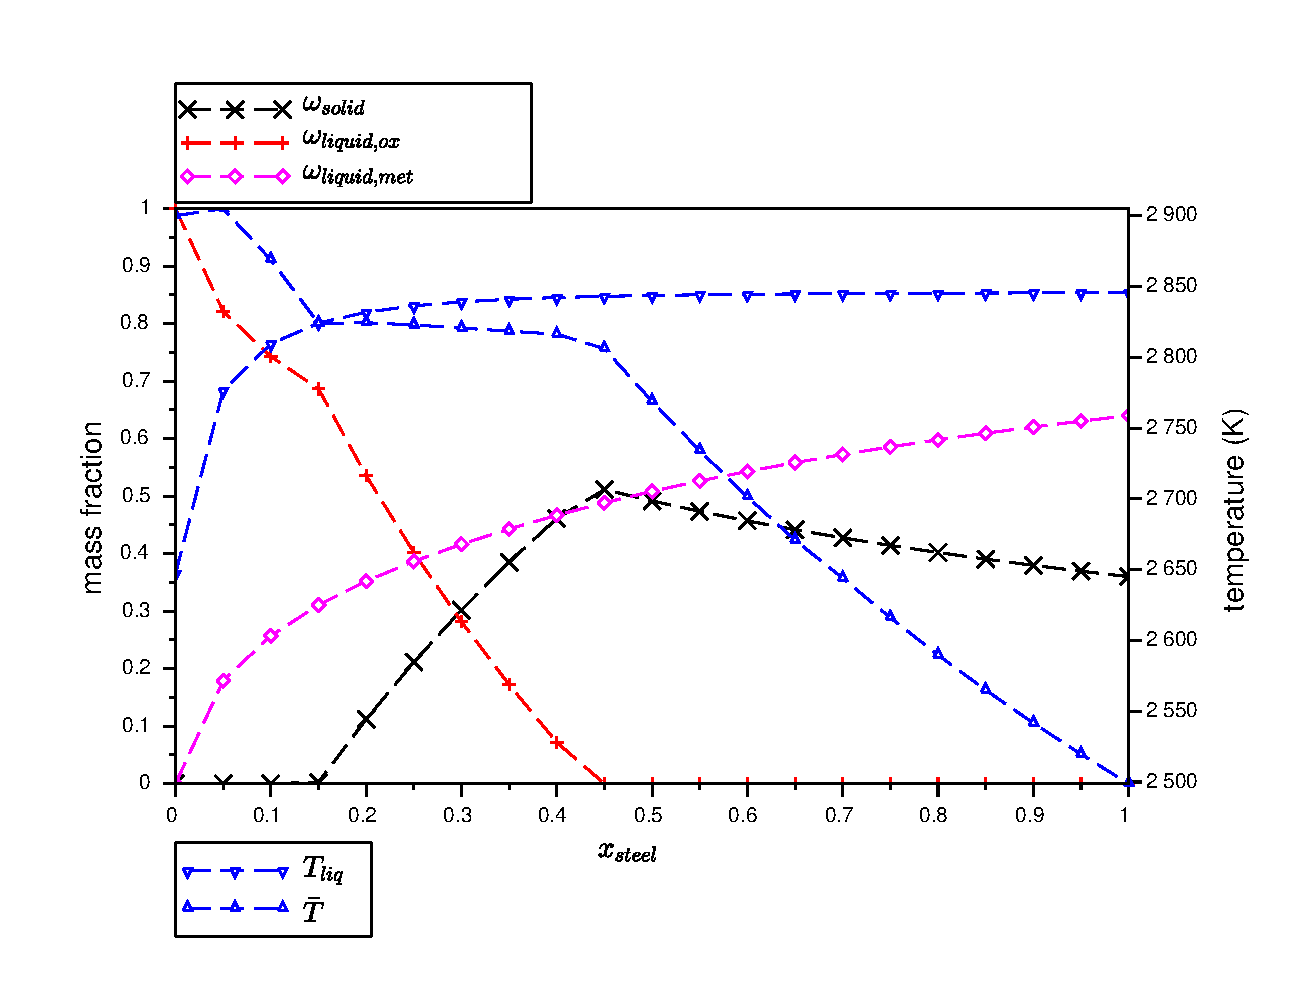
\includegraphics[width=\textwidth]{figures/CalphadBasedEOSTest/OpenCalphad_NUCLEA9_eq/C32_1850_x-T.eps} 
\caption{\T{equilibrium} case} \label{fig:x-T_C32_1850_OpenCalphad_NUCLEA9_eq} 
\end{subfigure}
\hspace{0.01\textwidth}%
\begin{subfigure}[t]{0.48\textwidth}
 \centering 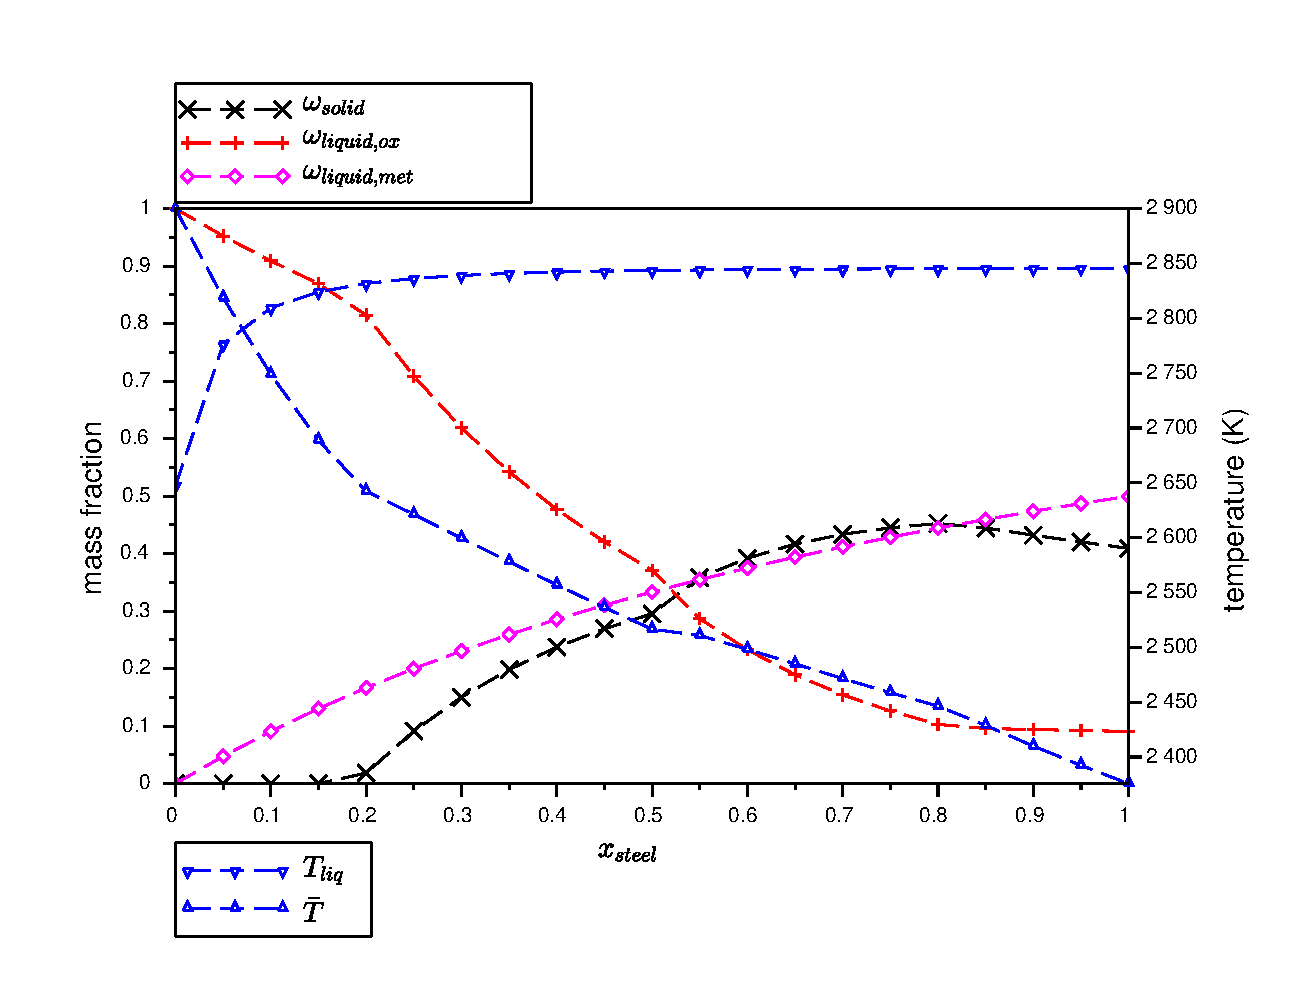
\includegraphics[width=\textwidth]{figures/CalphadBasedEOSTest/OpenCalphad_NUCLEA9_separatedEqs/C32_1850_x-T.eps} 
\caption{\T{independent systems} case} \label{fig:x-T_C32_1850_OpenCalphad_NUCLEA9_separatedEqs} 
\end{subfigure}
\\
\begin{subfigure}[t]{0.48\textwidth} 
 \centering 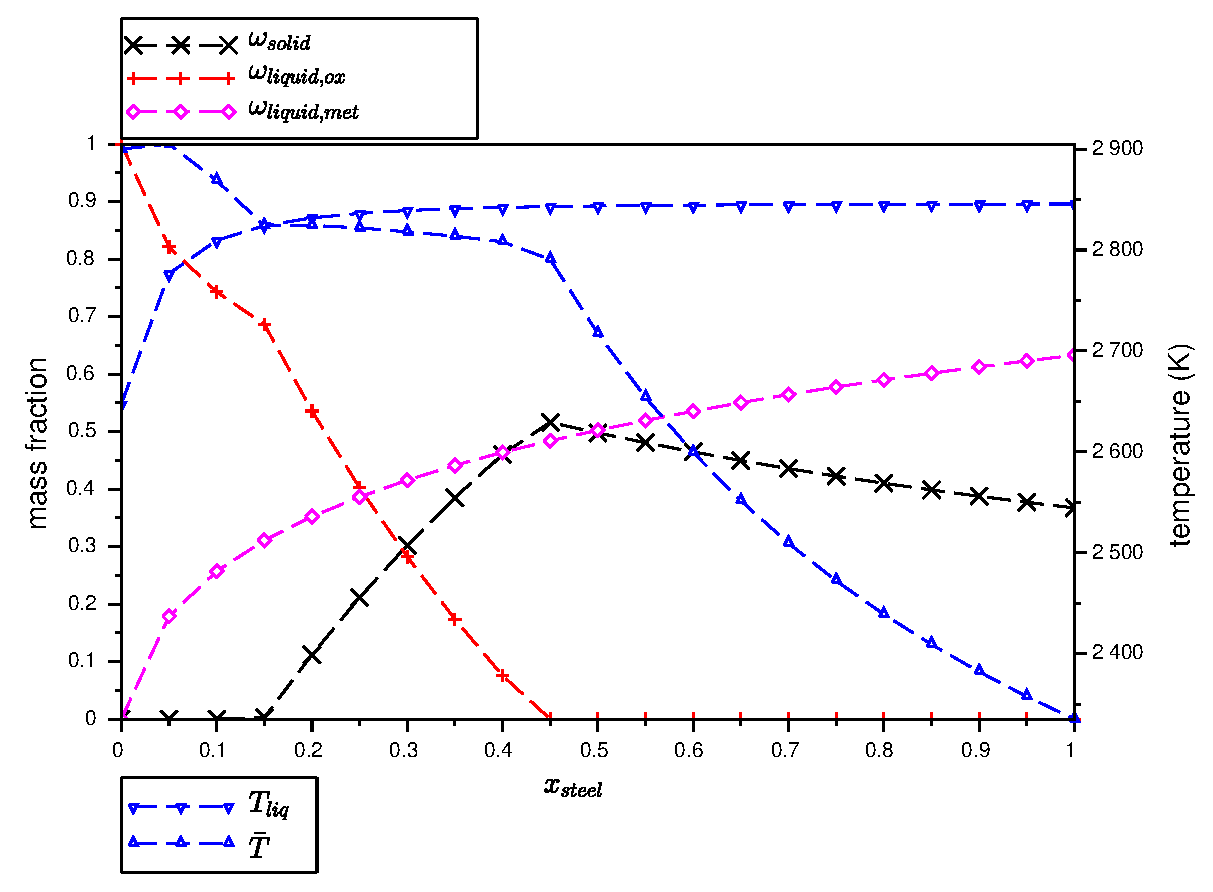
\includegraphics[width=\textwidth]{figures/CalphadBasedEOSTest/OpenCalphad_NUCLEA9_scheilGulliver/C32_1850_x-T.eps} 
\caption{\T{Scheil\-/Gulliver} case} \label{fig:x-T_C32_1850_OpenCalphad_NUCLEA9_scheilGulliver} 
\end{subfigure}
\hspace{0.01\textwidth}%
\begin{subfigure}[t]{0.48\textwidth} 
 \centering 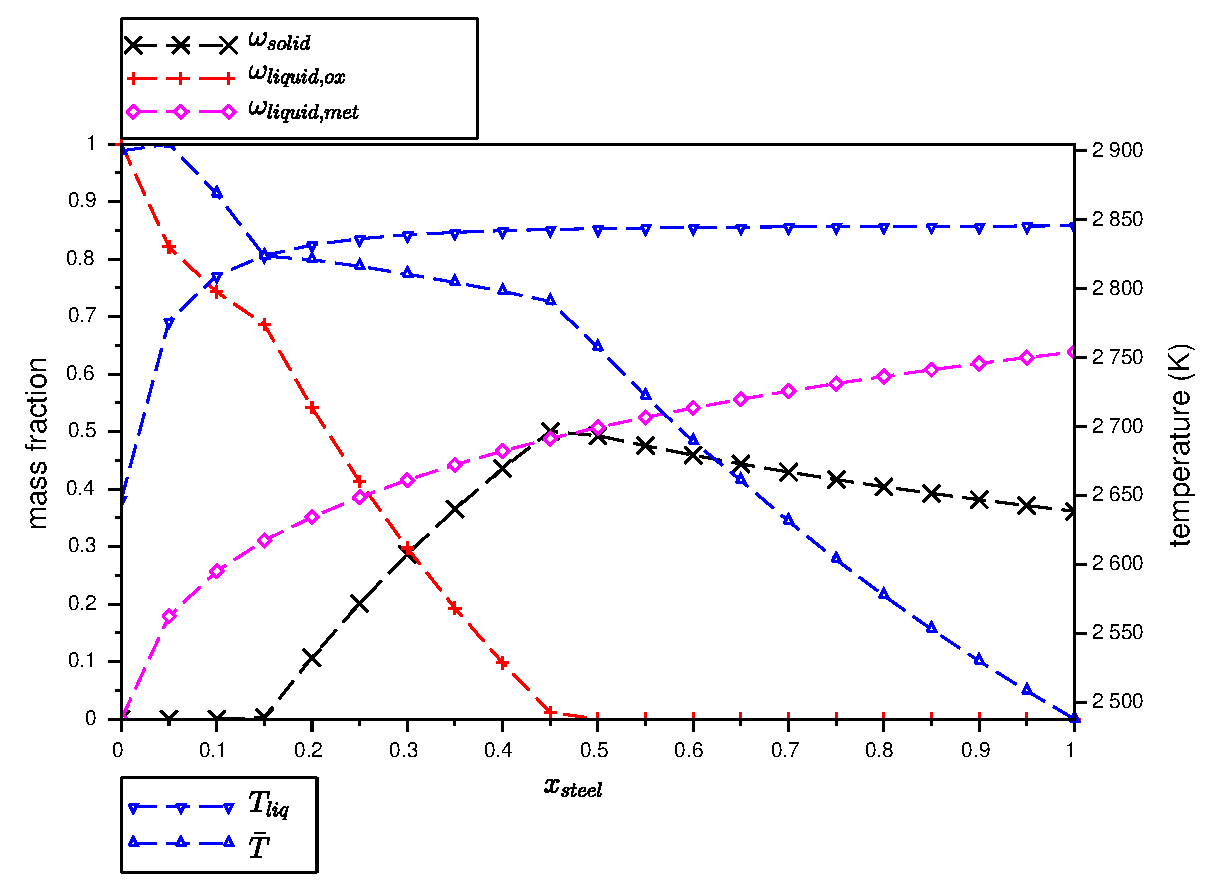
\includegraphics[width=\textwidth]{figures/CalphadBasedEOSTest/OpenCalphad_NUCLEA9_separatedLiquidEqs/C32_1850_x-T.eps} 
\caption{\T{independent solidification} case} \label{fig:x-T_C32_1850_OpenCalphad_NUCLEA9_separatedLiquidEqs} 
\end{subfigure}
\\
\begin{subfigure}[t]{1.0\textwidth}
% \hskip 0.01\textwidth
\begin{tabular}{cc}
   \begin{minipage}[b]{0.48\textwidth}
   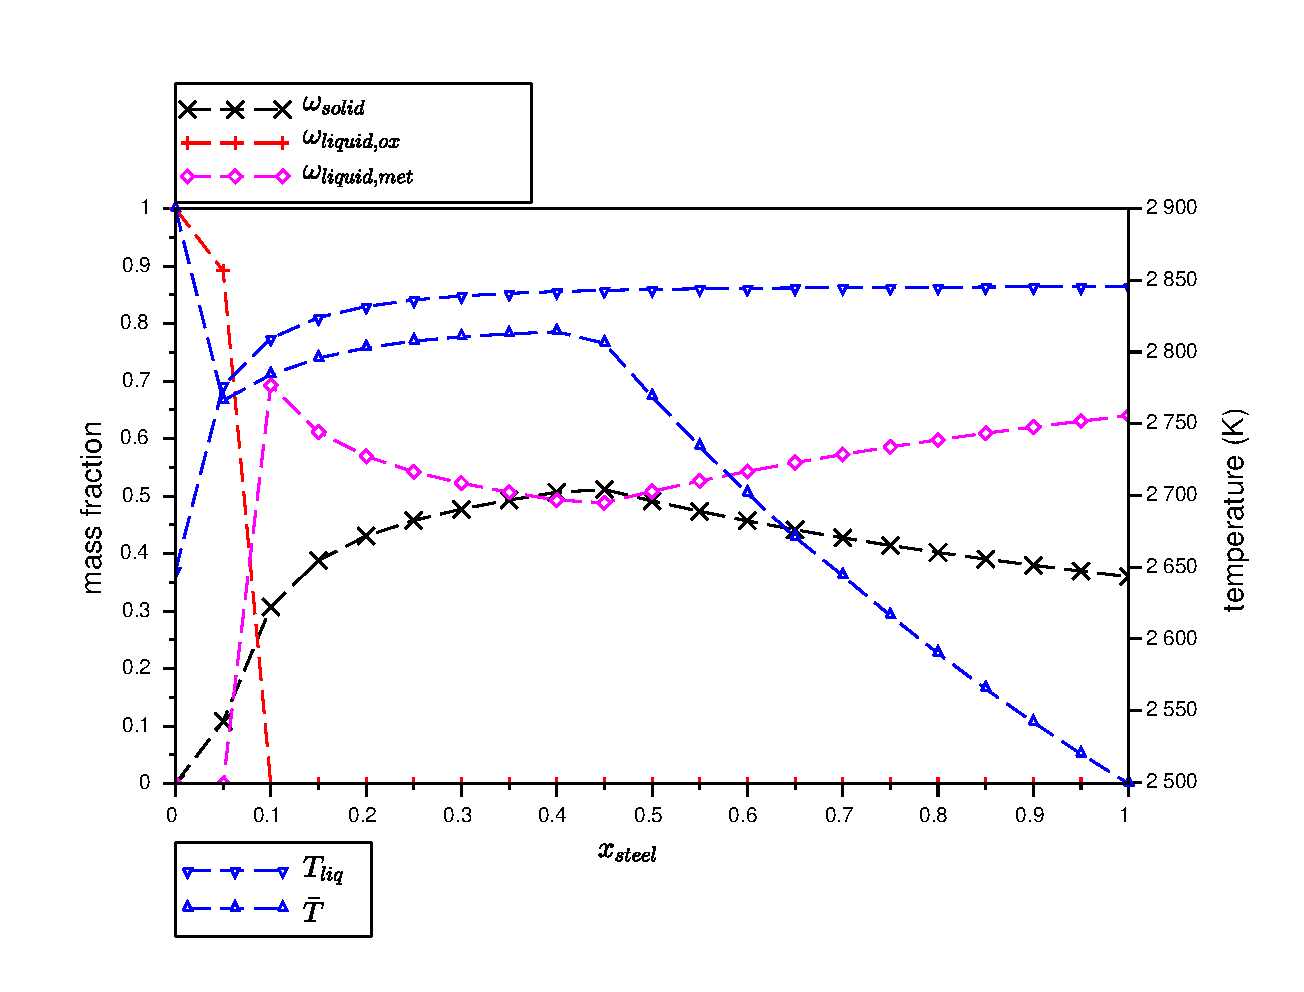
\includegraphics[width=\textwidth]{figures/CalphadBasedEOSTest/OpenCalphad_NUCLEA9_eq_noLiquidSeparation/C32_1850_x-T.eps} 
   \end{minipage}
 & \begin{minipage}[b]{0.48\textwidth} 
 In this case, only one liquid phase is present throughout the sequence. However, we have kept the same plot features as in the other cases in such a way that for $x_{steel} \in ]0.05, 0.1[$, the nature (``oxidic'' or ``metallic'') of the liquid phase is changed according to the criterion we have used so far. \\~\\~\\
 \end{minipage}
\end{tabular}
\caption{\T{single liquid equilibrium} case} \label{fig:x-T_C32_1850_OpenCalphad_NUCLEA9_eq_noLiquidSeparation} 
\end{subfigure}
\caption{$\bar{\temperature{}}$, $\temperature{liq}$ and $\omega_\gamma$ as a function of $x_{steel}$ for the different computational cases} \label{fig:x-T_C32_1850} 
\end{figure}

\subsubsection{Conclusions and recommendations}

As discussed previously, results reported in \cite{Bakouta2015} have shown that the adequate closure of conservation equations for a multilayer in-vessel corium behavior model is an issue when thermochemical interactions are considered. Consistency in terms of thermodynamical hypotheses between these closure relationships and thermochemical modeling should be ensured as far as possible and, at least, when the associated impact on the overall model is important. In this context, the following recommendations for the EOS construction can be drawn from this benchmark.

First of all, the important impact of steel-corium interaction on the EOS is confirmed. In addition, consistency with thermochemical modeling of interacting metal and oxidic phases rules out the simplified approach (\T{independent systems} option) used in some codes.

Then, the impact of liquid separation at equilibrium on the EOS cannot be neglected and neither \T{equi\-librium} nor \T{single liquid equilibrium} options offer an adequate general solution. The \T{single liquid equilibrium} option is not thermodynamically consistent while assuming instantaneous equilibrium (\T{equi\-librium} option) may not be coherent with the coupling to thermochemical kinetic models. Actually, constructing an EOS that treats adequately and in a general way the liquid miscibility gap in this context appears as impossible. As a consequence, the liquid phase separation related to this liquid miscibility gap should be explicitly modeled ``out of '' the EOS on a case-by-case basis depending on the conditions of thermochemical interaction between liquid molten steel and suboxidized corium. 
 
\begin{remark}
 Note that, in many cases, the macroscopic conservation equations are written over spatial zones that have an overall composition out of such a miscibility gap and this problem is not raised. For instance, it can be so for a multilayer corium pool model assuming that the hydrodynamic separation of liquid phases is always fast in comparison with other phenomena. In this case, it requires the explicit treatment of all possible molten steel and suboxidized corium interactions (depending on molten steel relocation hypotheses in the corium lower head modeling). Only an inter-layer mass transfer model (such as \cite{LeTellier2014} implemented in PROCOR and MAAP-EDF) is needed when steel is supposed to always relocate on top of the oxidic pool as in the PROCOR model. However, when steel migration through the crust to the oxidic pool is taken into account , an explicit model of the related thermochemical interaction should be introduced in such a way that, neglecting the hydrodynamic transient, the steel components relocation on top and/or bottom of the oxidic layer is calculated.
\end{remark}

Finally, the different options related to the solidification path have a more limited impact in the limited range of composition and temperature covered in this benchmark. In any case, from the point of view of the EOS construction, they do not induce additional difficulties. Note that, taking into account a possible solid phase fraction in the liquid layer bulk requires further modifications of the thermal modeling; at least, the dynamic viscosity model will have to be modified along with some heat transfer closure laws.


%%%%%%%%%%%%%%%%%%%%%%%%%%%%%%%%%%%%%%%%%%%%%%%%%%%%%%%%%%%%%%%%%%%%%%%%%%%%%
\section{Sampling, storage and interpolation of CALPHAD-based thermodynamic properties} \label{sect:practical}
%%%%%%%%%%%%%%%%%%%%%%%%%%%%%%%%%%%%%%%%%%%%%%%%%%%%%%%%%%%%%%%%%%%%%%%%%%%%%

%%%%%%%%%%%%%%%%%%%%%%%%%%%%%%%%%%%%%%%%%%%%%%%%%%%%%%%%%%%%%%%%%%%%%%%%%%%%%
\section{Conclusions and perspectives} \label{sect:concl}
%%%%%%%%%%%%%%%%%%%%%%%%%%%%%%%%%%%%%%%%%%%%%%%%%%%%%%%%%%%%%%%%%%%%%%%%%%%%%

\section*{Acknowledgments}

\section*{References}
\bibliography{../../References/lma-jabref}

\end{document}
